\section{研究进展以及存在的问题}
\subsection{学术成果}
以下是目前的研究成果:
\begin{itemize}
    \item 论文题目:Image Computation for Quantum Transition Systems
    \begin{itemize}
        \item ICCAD 2023 投稿情况:
        \begin{itemize}
            \item 论文编号:568
            \item 审稿结果:投稿被拒
            \item 审稿人评分:2,4,4
        \end{itemize}
        \item DAC2024 投稿情况:
        \begin{itemize}
            \item 当前状态:在投
            \item 预期反馈日期:2024年2月26日前
        \end{itemize}
    \end{itemize}
\end{itemize}
\subsection{研究内容进展}
在模型检测中,image computation指的是在给定当前状态$s_i\in S$和行为$\alpha\in Act$的情况下计算接下来的状态。
目前,关于使用TDD对量子的image computation的计算已经完成。图\ref{fig:grover-compare}表示了对Grover搜索算法运行不同image computation算法的资源对比。图\ref{fig:QFT-compare}表示了对quantum Fourier transform(QFT)算法运行不同image computation算法的资源对比。图\ref{fig:BV-compare}表示了对Bernstein–Vazirani(BV)算法运行不同image computation算法的资源对比。图\ref{fig:GHZ-compare}表示了对Greenberger–Horne–Zeilinger (GHZ)状态制备电路运行不同image computation算法的资源对比。图\ref{fig:QRW-compare}表示了对在$2^n$ 环上的quantum random walk (QRW)算法运行不同image computation算法的资源对比。
\begin{figure}[!htbp]
    \centering
    \begin{subfigure}[b]{.4\textwidth}
        \centering
        \includegraphics[height=4cm]{Img/alg_Grover_time.pdf}
        \caption{对Grover 算法应用不同电路拆分技术的时间对比}
        \label{fig:grover-time}
    \end{subfigure}
    \qquad
    \begin{subfigure}[b]{.4\textwidth}
        \centering
        \includegraphics[height=4cm]{Img/alg_Grover_node.pdf}
        \caption{对Grover 算法应用不同电路拆分技术的最大节点对比}
        \label{fig:grover-node}
    \end{subfigure}
    
    \caption{对Grover算法运行image computation时不同电路拆分技术的资源对比}
    \label{fig:grover-compare}
\end{figure}
\begin{figure}[!htbp]
    \centering
    \begin{subfigure}[b]{.4\textwidth}
        \centering
        \includegraphics[height=4cm]{Img/alg_QFT_time.pdf}
        \caption{对QFT 算法应用不同电路拆分技术的时间对比}
        \label{fig:QFT-time}
    \end{subfigure}
    \qquad
    \begin{subfigure}[b]{.4\textwidth}
        \centering
        \includegraphics[height=4cm]{Img/alg_QFT_node.pdf}
        \caption{对QFT 算法应用不同电路拆分技术的最大节点对比}
        \label{fig:QFT-node}
    \end{subfigure}
    \caption{对QFT算法运行image computation时不同电路拆分技术的资源对比}
    \label{fig:QFT-compare}
\end{figure}
\begin{figure}[!htbp]
    \centering
    \begin{subfigure}[b]{.4\textwidth}
        \centering
        \includegraphics[height=4cm]{Img/alg_BV_time.pdf}
        \caption{对BV 算法应用不同电路拆分技术的时间对比}
        \label{fig:BV-time}
    \end{subfigure}
    \qquad
    \begin{subfigure}[b]{.4\textwidth}
        \centering
        \includegraphics[height=4cm]{Img/alg_BV_node.pdf}
        \caption{对BV 算法应用不同电路拆分技术的最大节点对比}
        \label{fig:BV-node}
    \end{subfigure}
    \caption{对BV算法运行image computation时不同电路拆分技术的资源对比}
    \label{fig:BV-compare}
\end{figure}
\begin{figure}[!htbp]
    \centering
    \begin{subfigure}[b]{.4\textwidth}
        \centering
        \includegraphics[height=4cm]{Img/alg_GHZ_time.pdf}
        \caption{对GHZ 算法应用不同电路拆分技术的时间对比}
        \label{fig:GHZ-time}
    \end{subfigure}
    \qquad
    \begin{subfigure}[b]{.4\textwidth}
        \centering
        \includegraphics[height=4cm]{Img/alg_GHZ_node.pdf}
        \caption{对GHZ 算法应用不同电路拆分技术的最大节点对比}
        \label{fig:GHZ-node}
    \end{subfigure}
    \caption{对GHZ算法运行image computation时不同电路拆分技术的资源对比}
    \label{fig:GHZ-compare}
\end{figure}
\begin{figure}[!htbp]
    \centering
    \begin{subfigure}[b]{.4\textwidth}
        \centering
        \includegraphics[height=4cm]{Img/alg_QRW_time.pdf}
        \caption{对QRW 算法应用不同电路拆分技术的时间对比}
        \label{fig:QRW-time}
    \end{subfigure}
    \qquad
    \begin{subfigure}[b]{.4\textwidth}
        \centering
        \includegraphics[height=4cm]{Img/alg_QRW_node.pdf}
        \caption{对QRW 算法应用不同电路拆分技术的最大节点对比}
        \label{fig:QRW-node}
    \end{subfigure}
    \caption{对QRW算法运行image computation时不同电路拆分技术的资源对比}
    \label{fig:QRW-compare}
\end{figure}

表\ref{table:time}给出了在不同电路拆分技术下具体的各类算法的计算时间,单位为秒,max node表示计算过程中TDD的节点最大个数。
其中basic表示没有使用优化技术,addition表示使用研究方法\ref{addition}的addition优化技术,contraction表示使用研究方法\ref{contraction}中的contraction优化技术。“-”表示超过一小时的运行上限。
\begin{table}[!htbp]
    \centering
    \begin{tabular}{llllllllll}
        \hline
        \multirow{2}{*}{Benchmark} &  & \multicolumn{2}{c}{basic} &  & \multicolumn{2}{c}{addition} &  & \multicolumn{2}{c}{contraction} \\ \cline{3-4} \cline{6-7} \cline{9-10} 
                                   &  & time        & max \#node       &  & time          & max \#node        &  & time           & max \#node          \\ \hline
        Grover\_15 &   & 19.33  & 15785     &   & 17.35      & 15099  & & 1.61 & 597  \\
        Grover\_18 &   & 76.47  & 61694     &   & 66.02      & 60332  & & 2.41 & 516  \\
        Grover\_20 &   & 294.65 & 243946    &   & 259.87     & 241240 & & 4.39  & 1036 \\ 
        Grover\_40 &   & -      &           &   & -          &        & & 2953.57 & 851973 \\
        \hline
        QFT\_15     &  & 34.64   & 65536   &  & 18.88  & 32770   &  & 0.08 & 63  \\
        QFT\_18     &  & 282.12  & 524288  &  & 148.13 & 262146 &   & 0.10  & 31  \\
        QFT\_20     &  & 1199.21 & 2097152 &  & 655.19 & 1048578 &  & 0.12 & 63  \\
        QFT\_30     &  & -       &         &  & -      &        &  & 0.29 & 31  \\
        QFT\_50     &  & -       &         &  & -      &        &  & 1.02 & 51  \\
        QFT\_100    &  & -       &         &  & -      &        &  & 7.14 & 101 \\
        \hline
        BV\_100     &  & 7.36    & 596     &  & 7.43      & 596     &  & 0.41           & 102 \\
        BV\_200     &  & 31.57   & 1196    &  & 30.03     & 1196    &  & 1.70           & 202 \\
        BV\_300     &  & 75.66   & 1796    &  & 75.56     & 1796    &  & 4.28           & 302 \\
        BV\_400     &  & 146.47  & 2396    &  & 145.40    & 2396    &  & 9.18           & 402 \\
        BV\_500     &  & 244.15  & 2996    &  & 223.90    & 2996    &  & 16.31          & 502 \\
        \hline
        GHZ\_100    &  & 0.38    & 595     &  & 0.13      & 301    &  & 0.18           & 200 \\%& 0.03    
        GHZ\_200    &  & 0.72    & 1195    &  & 0.37      & 601    &  & 0.48           & 400 \\%& 0.12     
        GHZ\_300    &  & 1.29    & 1795    &  & 0.62      & 901    &  & 0.80           & 600 \\%& 0.24     
        GHZ\_400    &  & 2.03    & 2395    &  & 1.00      & 1201    &  & 1.26           & 800 \\%& 0.42     
        GHZ\_500    &  & 2.96    & 2995    &  & 1.45      & 1501    &  & 1.72           & 1000\\%& 0.62     
        \hline
        QRW\_15     &  & 36.86   & 13122     &  & 24.59     & 10882     & & 7.16  & 222 \\
        QRW\_18     &  & 139.76  & 90538     &  & 84.69     & 37064     & & 11.23 & 226 \\
        QRW\_20     &  & 341.05  & 265614    &  & 218.29    & 107714    & & 14.31 & 404 \\
        QRW\_30     &   &-       &          &  &-          &          & & 36.82 & 404 \\
        QRW\_50     &   &-       &          &  &-          &          & & 118.08 & 404 \\
        QRW\_100    &   &-       &          &  &-          &          & & 692.08 & 436 \\
        \hline
    \end{tabular}
    \caption{对不同测试实验应用image computation}
    \label{table:time}
\end{table}

通过对比不同优化技术下的计算时间,可以看到使用优化技术能够显著降低计算时间。例如,在Grover-20的例子中,使用"contraction"优化技术的情况下,计算时间从294秒降低到了4秒。这表明优化技术在提高计算效率方面起到了积极的作用。

同时,表\ref{table:addition}展示了对同一线路,即Grover\_15应用不同的addition参数的时间,可以看到合适的参数选择也是非常重要的。
\begin{table}[!htbp]
    \centering
    \begin{tabular}{c|ccccccccccccccc}
        \rowcolor[HTML]{FFFFFF} 
        \diagbox{k1}{k2}                         & 1                           & 2                           & 3                           & 4                           & 5                           & 6                           & 7                          & 8                           & 9                           & 10                          & 11                          & 12                          & 13                          & 14                          & 15                          \\\hline
            \rowcolor[HTML]{FFFFFF} 
    1                          & 2.8                                              & 2.2                         & 2.1                         & \cellcolor[HTML]{CCC0DA}2.0 & \cellcolor[HTML]{CCC0DA}1.9 & \cellcolor[HTML]{CCC0DA}2.0                      & 2.1                        & \cellcolor[HTML]{CCC0DA}2.0 & 2.1                         & \cellcolor[HTML]{CCC0DA}2.0 & \cellcolor[HTML]{CCC0DA}2.0 & 2.1                         & 2.2                         & 2.1                         & 2.1                         \\ \cline{3-7}
    \rowcolor[HTML]{CCC0DA} 
    
    \rowcolor[HTML]{FFFFFF} 
    3                          & \multicolumn{1}{l|}{\cellcolor[HTML]{FFFFFF}2.2} & \cellcolor[HTML]{CCC0DA}1.9 & \cellcolor[HTML]{CCC0DA}1.8 & \cellcolor[HTML]{CCC0DA}1.6 & \cellcolor[HTML]{CCC0DA}2.0 & \multicolumn{1}{l|}{\cellcolor[HTML]{CCC0DA}1.9} & 2.1                        & 2.1                         & 2.5                         & 2.3                         & 2.7                         & 2.3                         & 3.1                         & 2.8                         & 3.3                         \\
    \rowcolor[HTML]{FFFFFF} 
    4                          & \multicolumn{1}{l|}{\cellcolor[HTML]{FFFFFF}2.3} & \cellcolor[HTML]{CCC0DA}1.8 & \cellcolor[HTML]{CCC0DA}2.0 & \cellcolor[HTML]{CCC0DA}1.7 & \cellcolor[HTML]{CCC0DA}2.0 & \multicolumn{1}{l|}{\cellcolor[HTML]{FFFFFF}2.1} & 2.2                        & 2.1                         & 2.6                         & 2.3                         & 2.8                         & 2.7                         & 3.3                         & 3.0                         & 3.3                         \\
    \rowcolor[HTML]{FFFFFF} 
    5                          & \multicolumn{1}{l|}{\cellcolor[HTML]{FFFFFF}2.2} & \cellcolor[HTML]{CCC0DA}1.7 & \cellcolor[HTML]{CCC0DA}1.9 & \cellcolor[HTML]{CCC0DA}1.6 & \cellcolor[HTML]{CCC0DA}1.9 & \multicolumn{1}{l|}{\cellcolor[HTML]{CCC0DA}2.0} & 2.3                        & \cellcolor[HTML]{CCC0DA}1.9 & 2.5                         & 2.3                         & 2.8                         & 2.7                         & 3.4                         & 3.0                         & 3.6                         \\
    \rowcolor[HTML]{FFFFFF} 
    6                          & \multicolumn{1}{l|}{\cellcolor[HTML]{FFFFFF}2.1} & \cellcolor[HTML]{B1A0C7}1.5 & \cellcolor[HTML]{CCC0DA}1.8 & \cellcolor[HTML]{CCC0DA}1.7 & 2.2                         & \multicolumn{1}{l|}{\cellcolor[HTML]{CCC0DA}1.9} & 2.5                        & 2.2                         & 2.9                         & 2.8                         & 3.1                         & 2.9                         & 3.7                         & 3.7                         & 4.2                         \\
    \rowcolor[HTML]{FFFFFF} 
    7                          & \multicolumn{1}{l|}{\cellcolor[HTML]{FFFFFF}2.1} & \cellcolor[HTML]{CCC0DA}1.5 & \cellcolor[HTML]{CCC0DA}1.9 & \cellcolor[HTML]{CCC0DA}1.6 & 2.2                         & \multicolumn{1}{l|}{\cellcolor[HTML]{CCC0DA}1.9} & 2.5                        & 2.2                         & 2.8                         & 3.0                         & 3.6                         & 3.3                       & 4.2                         & 5.7                         & 5.0                         \\
    \rowcolor[HTML]{FFFFFF} 
    8                          & \multicolumn{1}{l|}{\cellcolor[HTML]{CCC0DA}2.0} & \cellcolor[HTML]{CCC0DA}1.7 & \cellcolor[HTML]{CCC0DA}1.8 & \cellcolor[HTML]{CCC0DA}1.7 & 2.1                         & \multicolumn{1}{l|}{\cellcolor[HTML]{CCC0DA}2.0} & 2.4                        & 2.2                         & 2.8                         & 2.8                         & 3.7                         & 3.4                         & 4.3                         & 4.8                         & 5.2                         \\
    \rowcolor[HTML]{FFFFFF} 
    9                          & \multicolumn{1}{l|}{\cellcolor[HTML]{FFFFFF}2.1} & \cellcolor[HTML]{B1A0C7}1.5 & \cellcolor[HTML]{CCC0DA}2.0 & \cellcolor[HTML]{B1A0C7}1.4 & 2.2                         & \multicolumn{1}{l|}{\cellcolor[HTML]{CCC0DA}2.0} & 2.5                        & \cellcolor[HTML]{CCC0DA}2.0 & 3.3                         & 2.9                         & 3.7                         & 3.5                         & 4.9                         & 4.7                         & 5.8                         \\ \cline{3-7}
    \rowcolor[HTML]{FFFFFF} 
    10                         & 2.3                                              & \cellcolor[HTML]{CCC0DA}1.9 & 2.3                         & \cellcolor[HTML]{CCC0DA}1.6 & 2.6                         & 2.7                                              & 3.1                        & 2.2                         & 4.0                         & 3.6                         & 4.6                         & 3.9                         & 5.6                         & 5.2                         & 7.5                         \\
    \rowcolor[HTML]{FFFFFF} 
    11                         & 3.2                                              & 3.2                         & 3.5                         & 3.1                         & 4.7                         & 4.2                                              & 5.6                        & 4.2                         & 6.8                         & 7.2                         & 7.6                         & 6.3                         & 9.0                         & 8.1                         & \cellcolor[HTML]{8DB4E2}11  \\
    \rowcolor[HTML]{FFFFFF} 
    12                         & 5.6                                              & 6.0                         & 7.2                         & 6.0                         & 8.3                         & 9.0                                              & 8.9                        & 7.8                         & \cellcolor[HTML]{8DB4E2}11  & \cellcolor[HTML]{8DB4E2}11  & \cellcolor[HTML]{8DB4E2}12  & \cellcolor[HTML]{8DB4E2}11  & \cellcolor[HTML]{8DB4E2}12  & \cellcolor[HTML]{8DB4E2}15  & \cellcolor[HTML]{8DB4E2}16  \\
    \rowcolor[HTML]{8DB4E2} 
    \cellcolor[HTML]{FFFFFF}13 & 11                                               & 12                          & 14                          & 12                          & 15                          & 18                                               & 18                         & 15                          & 18                          & 20                          & 18                          & 32                          & 32                          & 30                          & 25                          \\
    \rowcolor[HTML]{8DB4E2} 
    \cellcolor[HTML]{FFFFFF}14 & 20                                               & 21                          & 24                          & 32                          & 31                          & 44                                               & 77                         & 50                          & 86                          & \cellcolor[HTML]{538DD5}109 & 68                          & \cellcolor[HTML]{538DD5}133 & 70                          & \cellcolor[HTML]{538DD5}119 & \cellcolor[HTML]{538DD5}142 \\
    \rowcolor[HTML]{538DD5} 
    \cellcolor[HTML]{FFFFFF}15 & \cellcolor[HTML]{8DB4E2}28                       & \cellcolor[HTML]{8DB4E2}30  & \cellcolor[HTML]{8DB4E2}31  & \cellcolor[HTML]{8DB4E2}53  & \cellcolor[HTML]{8DB4E2}69  & 111                                              & \cellcolor[HTML]{8DB4E2}85 & \cellcolor[HTML]{8DB4E2}81  & 102                         & 153                         & 114                         & 130                         & 166                         & 162                         & 235                        
                     
    \end{tabular}
    \caption{对grover\_15应用不同的addition 参数}%calculating the 
    \label{table:addition}
\end{table}
  
在技术实现上,构建了两个版本的量子线路转化为TDD的工具,分别基于C语言和Python语言。这些工具的开发对于实现我们的研究方法至关重要,提高了实验的灵活性和效率。
其中的C语言的TDD
\begin{figure}[!htbp]
    \centering
    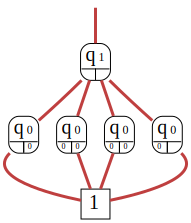
\includegraphics[width=.8\textwidth]{Img/cnot.pdf}
\end{figure}

\subsection{学术论文进展}
在学术论文撰写方面的进展包括:
\begin{itemize}
    \item 完成了学术论文中关于研究背景的详细调查和综述,这部分内容主要包括了量子模型检测的背景知识与重要性。
    \item 撰写了研究内容的方法论部分,详细描述了主要的研究方法和实验设计。阐述了我们的研究方法,并详细介绍了方法的实施步骤和预期目标。
\end{itemize}
\subsection{目前存在的问题}
在本研究过程中,主要遇到了两个问题,这些问题对研究的深入发展和实际应用产生了重要影响。


首先,面临的一个关键挑战是如何将所提出的方法扩展应用到更大规模的实例。这不仅涉及到算法的效率问题,还包括数据处理能力的提升。对于实现验
证量子计算算法在更广泛领域的应用至关重要。为了解决这一挑战,目前采用电路拆分方法来降低 TDD 的资源消耗,并挖掘可能的并行计算机会。此外,还计划应用更灵活的索引策略和 limdd 的思路,以期达到更高效的处理效果。

其次,另一个重要的问题是如何将研究方法应用于更加实用的示例。这是将理论研究转化为实际应用的关键一步。目前考虑的主要方向是将此方法应用到
量子线路设计,即 QDA(Quantum Design Automation)领域。计划未来能够将本研究成果应用于不同的 synthesis 算法的验证等价性中,从而在量子计算的实际应用中发挥更大的作用。